\chapter{Log and Checkpoint}

\section{Problems and Goals}
As for \textbf{recovery}, there are three ways
\begin{itemize}
    \item Replication. It is true that replication can make the system more secure, but it is expensive and also require a lot of synchronization work.
    \item Checkpoint. If the system make changes (progress), we can make checkpoints to store the system states. But the problem for checkpoint is that the systems need a \textbf{freeze} when backing up. However, we can try to find a consistent recovery line, which will be discussed later.
    \item Log. The classic technique is \textbf{Write Ahead Logging}. Events need to be written in the log first before executed.
\end{itemize}

For cooperation between checkpoint and log, we use logs between checkpoints. Recovery involves checkpointing and logging. Checkpoints store the state of process, logging involves recording the operations that produced the current state.

\section{Sender-based Logging}
Sender based logging is very important in those cases where receivers are thin or unreliable. In other words, we would want to log messages on the sender if the receiver does not have the resources to maintain the logs, or if the receiver is likely to fail. 

\subsubsection{Ensure that the order in both senders and receivers are correct.}

Senders can play back the logging in the same order in which they were dispatched.It is difficult to order the messages from senders in the receiver side.

To ensure this, we follow the protocol:
\begin{itemize}
    \item The sender logs a message and send it.
    \item The receiver gets the message and ACKs it with the time local to the receiver.
    \item The sender adds this timestamp in the ACK into that log entry.
\end{itemize}
Under this protocol, we can resend the message with the order recorded by the senders when dispatching. At the same time, when messages arrive the receivers, they can also order the messages with the receivers' time stamp.

\subsubsection{Ensure the sender get the timestamped ACKs from receivers (make sure logs are complete)}

Require the sender to send a ACK-ACK to the receiver before send a following message. 
\begin{figure}
\centering
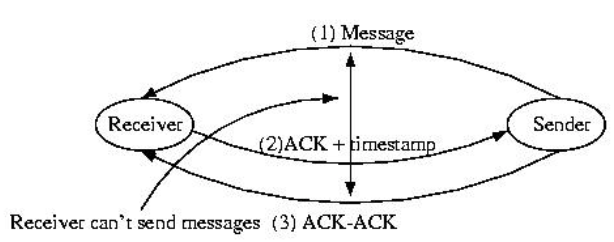
\includegraphics[width=\textwidth]{img/ch03-log_ackack.png}
\caption{ACK-ACK log.}
\label{fig:ch03-log_ackack}
\end{figure}

Before the receiver gets the ACK-ACK for the first message, it cannot send messages to the sender. It make sure that we get the correct order in the receiver side.

\section{Recovery from Failure}
Recovery involves sending lots of history messages. \textbf{Duplicate messages} are the messages sent to other normal systems. \textbf{Orphan messages} are that after a rollback some systems may receive the messages that the recovering system does not remember sending. Rollback to a fail system may causes another system to rollback, which is known as \textbf{cascading rollbacks}. Eventually the systems will reach a state where they can move forward together, which is known as \textbf{recovery line}. After a rollback, a system may duplicate output, or request the input again, which is called \textbf{studdering}.

\subsection{Incarnation Numbers}
\textbf{Incarnation} is the period between checkpoints. Rebooting a system or restarting a cooperating process results in a new incarnation. We can number these incarnations. This number can be used to eliminate duplicate messages.

When a system is reincarnated, it sends a message to the cooperating systems informing them of the new incarnation number. The incarnation number is also send out with all messages. Therefore, the receivers can determine whether or not it is a duplicate message.

\textbf{How the receiver handles the incarnation numbers?}
\begin{itemize}
    \item If the incarnation number of the message is less than the expected number, the message is a duplicate, so it should be discarded.
    \item If the incarnation number is in the message is greater than the expected number, the sender is recovering, so block accepting messages, until it informs us about its new incarnation number.
    \item If they are the same, accept the message.
\end{itemize}

\subsection{Checkpoint: consistency}
The checkpoints of all the servers are unnecessary consistent. Therefore, we need to find a maximum recovery line.

\subsubsection{Interval Dependency Graph (IDG)}
The graph is constructed by creating a node for each interval, and then connecting subsequent intervals on the same processor by constructing an edge from a predecessor to its successor. Then an edge is draw from each interval during which one or more messages were received to the interval or intervals during which the message(s) was or were sent.
\begin{figure}
\centering
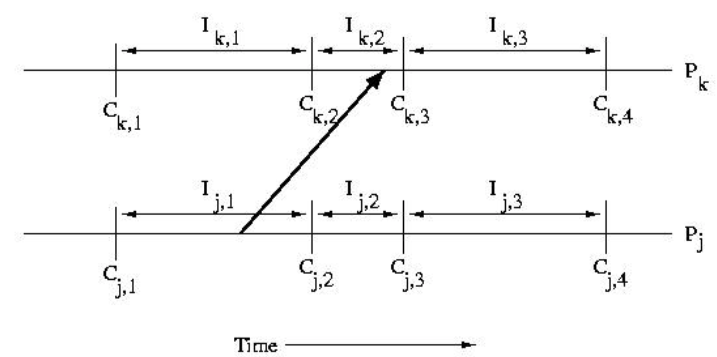
\includegraphics[width=\textwidth]{img/ch03-idg.png}
\caption{IDG}
\label{fig:ch03-idg}
\end{figure}

\textbf{Where to store the graph?} Each processor keeps the nodes and edges that are associated with it.

\textbf{How to find the recovery line?} If there are some lost intervals, the other servers rollback to a interval that is independent of the lost intervals. And this rollback continues until there is a recovery line established.

\subsubsection{Coordniated Checkpoints}
We can decrease the rollbacks happened in the whole system, by coordinating checkpoints. Actually we only discussed how to use IDG, but not how to implicitly form a IDG. Here is the discussion.

There are two methods:
\begin{itemize}
    \item Record message sequence number (the sender information). If the receiver gets a message, it send back a message to tell the senders to check if they checkpointed since the last time they sent the message. If not, the senders need to checkpoint in order to satisfy the dependency.
    \item Synchronized clock. Each processor creates a checkpoint every T units of time.
\end{itemize}

\section{Logging}

\subsection{Kinds of Logging}

\begin{itemize}
    \item Synchronous Logging. Logging before execution. It is expensive and slow.
    \item Asychronous Logging. Occasionally write the logs. Some messages may be logged, while others may not be logged.
\end{itemize}

\subsection{One Approach For Asychronous Logging: GDM}
First, the system maintains a \textbf{Global Dependency Matrix (GDM)}, each processor has a vector recording the interval numbers of processors it knows. 

\begin{figure}
\centering
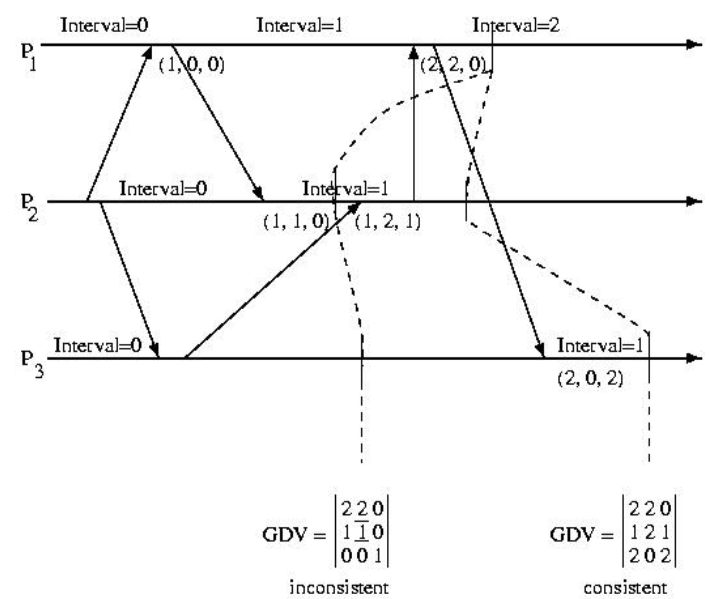
\includegraphics[width=\textwidth]{img/ch03-log_gdv.png}
\caption{GDM}
\label{fig:ch03-log_gdv}
\end{figure}

We can check if the matrix is consistent. The method is similar as before. You can check if the number on the processor's self is the greatest.

The method to find a new recovery line:
\begin{enumerate}
    \item Get the previous recovery line and new updates after the recovery line.
    \item Check for each update, if it can hold a consistent state for the system. If so, update the recovery line and go on checking.
\end{enumerate}

\subsection{Adaptive Logging}
We do not need to log every message. It only needs to log those messages that have originated from processors that have taken checkpoints more recently than it has. Before there are new updates existing on the senders. If the receiver is ahead, it won't worry about it and do not need to checkpoint.
